% Metódy inžinierskej práce

\documentclass[10pt,twoside,english,a4paper]{coursepaper}

\usepackage[english]{babel}
%\usepackage[T1]{fontenc}
\usepackage[IL2]{fontenc} % lepšia sadzba písmena Ľ než v T1
\usepackage[utf8]{inputenc}
\usepackage{graphicx}
\usepackage{url} % príkaz \url na formátovanie URL
\usepackage{hyperref} % odkazy v texte budú aktívne (pri niektorých triedach dokumentov spôsobuje posun textu)
\usepackage{copyrightbox}
\usepackage{caption}

\usepackage{cite}
\graphicspath{ {./images/} }
%\usepackage{times}
\newcommand{\source}[1]{\caption*{Source: {#1}} }

\pagestyle{headings}

\title{Loot boxes in video games and their link to problem gaming\thanks{Semestrálny projekt v predmete Metódy inžinierskej práce, ak. rok 2022/23, vedenie: MSc. Mirwais Ahmadzai}} % meno a priezvisko vyučujúceho na cvičeniach

\author{Jakub Bordáš\\[2pt]
	{\small Slovenská technická univerzita v Bratislave}\\
	{\small Fakulta informatiky a informačných technológií}\\
	{\small \texttt{xbordas@stuba.sk}}
	}

\date{\small 30. september 2022} % upravte



\begin{document}

\maketitle

\begin{abstract}
Loot boxes are crates in video games that contain randomised game content. Generally, adolescents are more prone to play video games. More than 2 billion people worldwide play video games for relaxation. To create more profit from their products, video game developers are implementing these loot boxes in their games. Every game in the TOP 5 leaderboard on SteamCharts.com (up to 04.10.2022) contains loot boxes. Creating more games with loot boxes creates an issue linking loot boxes with problem gambling. This article will focus more on the psychological features of loot boxes and how they should be regulated for young audiences or even deemed illegal.
\end{abstract}



\section{Introduction}

Motivujte čitateľa a vysvetlite, o čom píšete. Úvod sa väčšinou nedelí na časti.

Uveďte explicitne štruktúru článku. Tu je nejaký príklad.
Základný problém, ktorý bol naznačený v úvode, je podrobnejšie vysvetlený v časti~\ref{nejaka}.
Dôležité súvislosti sú uvedené v častiach~\ref{dolezita} a~\ref{dolezitejsia}.
Záverečné poznámky prináša časť~\ref{zaver}.



\section{What are loot boxes?} \label{sec:what}

\begin{figure*}[tbh]
	\centering
	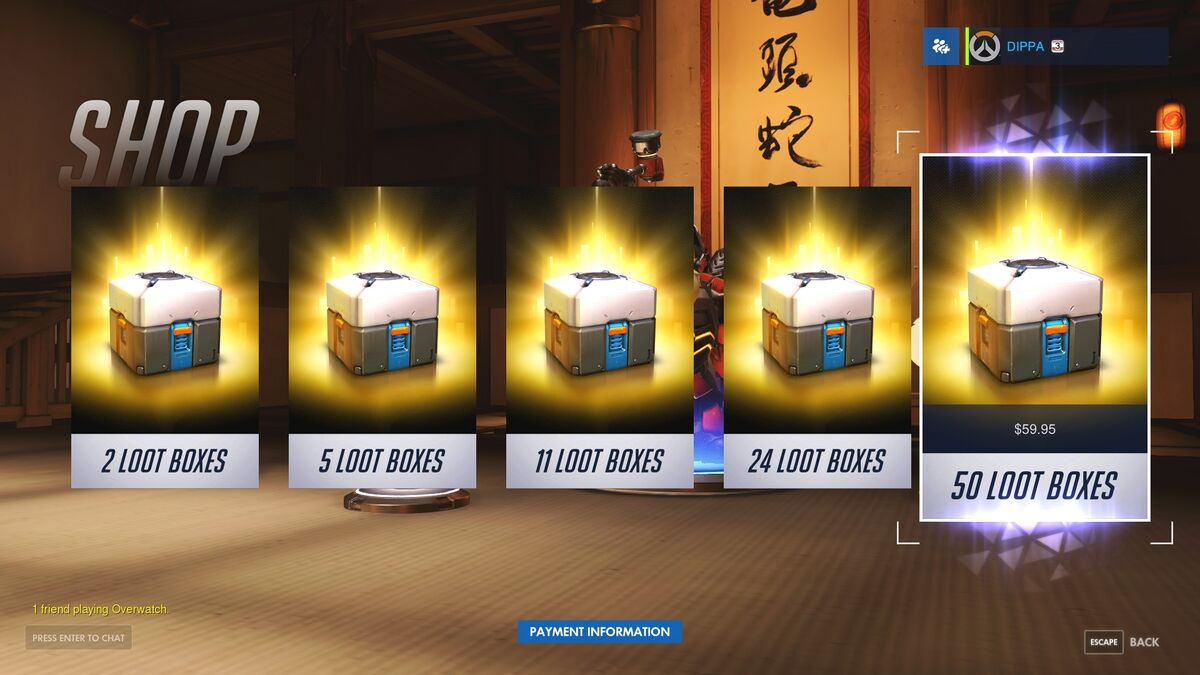
\includegraphics[scale=0.5]{img1}
	\caption{Loot boxes in Overwatch 1}
	\source{\url{https://crappygames.miraheze.org/wiki/Loot_box} }
	\label{fig:img1}
\end{figure*}

	Loot boxes are virtual containers in video games that contain one or more random rewards that alter the game in some way. Some can change avatar aesthetics, unlock new levels or improve in-game performance (e.g. via more powerful weapons or sets of armour). Possessing a unique avatar or powerful weapons is highly desirable. \par
	They are available for players to buy in popular games like Rocket League, Counter-Strike: Global Offensive, and League of Legends. Even more and more games tend to sell these loot boxes for real-world currency. In 2018 alone, they generated approximately \$30 billion\cite{juniper:revenue}. This strategy has become a leading business model for generating profit from video games. \par
	The spread of loot boxes has raised the question of whether they should be regulated as a form of gambling. According to an article by Mark D. Griffiths, many of the loot box characteristics match those of gambling. The basic idea behind gambling is that an individual stakes money on the outcome of a future event, which is determined by chance in the hopes of receiving the desired reward. This would not be a problem if most players were not young teenagers and adolescents. \par
	According to research\cite{springer:research} done on almost three thousand students in grades 7 to 12 in Ontario, most students (85\%) reported playing video games in the past year and almost 19\% reported playing video games daily. According to a more recent source\cite{theesa:facts}, a total of 66\% of Americans play video games regularly. 

\subsection{Features of loot boxes} \label{sec:features}

	Many games implement loot boxes in their way. Some may be more linked to the development of problem gambling than others. A few characteristics are listed below.

\begin{enumerate}

\item Loot boxes can give a player gameplay advantage

	Loot boxes in games like Counter-Strike: Global Offensive and Overwatch only contain cosmetic rewards and do not alter gameplay. However, not all games provide cosmetic-only rewards. For example, in FIFA's Ultimate Team mode players can pay to purchase 'player packs' that contain a random set of footballers. The rarer the footballer is, the better he performs in games.\cite{fifa:lootboxes}

\item Some loot boxes show missed rewards
	
\begin{figure*}[tbh]
	\centering
	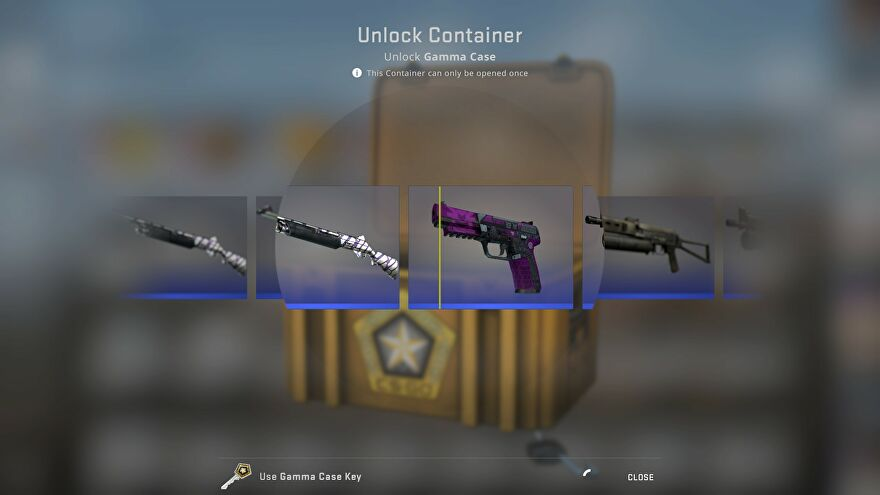
\includegraphics[scale=0.33]{img2}
	\caption{Opening loot boxes in Counter-Strike: Global Offensive}
	\source{\url{https://www.rockpapershotgun.com/senate-bill-fights-loot-boxes-and-pay-to-win} }
	\label{fig:img2}
\end{figure*}
	
	Counter-Strike: Global Offensive will show you which reward you got and all the near misses. This can trigger an emotion of nearly getting a legendary reward, but instead, you got a common one. This is not the case for all loot boxes.

\item Some loot boxes are given away for free

	In some games, you can only get loot boxes for real-world money. In other, however, you can get them for playing the game, completing in-game challenges, levelling up etc. For example, in Overwatch 1 you got one loot box for every level up. They could be purchased for real-world money, but you could get them for free. 

\item Some loot box rewards can be cashed out

	In many games, the rewards from loot boxes are bound to the player's account and cannot be cashed out or traded with other players. For example, in Overwatch or League of Legends, this is the case. However, in some games, these rewards can be re-sold to other players on the official marketplace. For example, in Counter-Strike: Global Offensive there is a slim chance you can get a rare knife. Because of their rarity, their price is enormous. For example, one variation of knife skin was once sold for over \$2000. \cite{csgo:knives}

\item Some loot boxes are time-limited
	
	In games like Overwatch 1, you could open specific types of loot boxes throughout the year. These special types contained different rewards from the regular ones. For example, there were Halloween, Christmas or Lunar New Year loot boxes. 

\end{enumerate}

\section{How to differentiate between gambling and other risk-related behaviour?} \label{sec:griffiths}

In\cite{gambling:characteristics}, Griffiths specifies five characteristics linked to gambling. These are:

\begin{enumerate}

\item The exchange of money or something of value.
\item A future event determines the results of this exchange, and the outcome of this event is unknown at the time that a bet is made.
\item Chance at least partly determines the outcome of the exchange.
\item Losses can be avoided by simply not taking part.
\item Winners gain at the sole expense of losers.

\end{enumerate}
	

\section{Loot boxes and their link to problem gaming} \label{sec:link}

	Analysis of 22 video games\cite{nature:psycho} that feature loot boxes showed that 10 of the 22 video games fulfilled all of the five characteristics of gambling specified by Griffiths \ref{sec:griffiths}.  They found that these games containing loot boxes  '100\% allow for (if not actively encourage) underage players to engage with these systems'. Young people exposed to gambling are more prone to developing problematic gambling behaviours\cite{springer:risks}. \par
	If loot boxes are linked to gambling, this would raise serious concerns about their availability to younger audiences. Given their features, the Dutch officials and government of the Netherlands have put a stop to loot boxes. This caused video game developers to alter their games and/or delete loot boxes entirely from these regions. This includes big video game studios like Activision Blizzard and Valve. Following this ban loot boxes should not be present in Belgium anymore. Unfortunately, this is not true. 82\% of the 100 highest-grossing iPhone games on the Belgian Apple Store still contain loot boxes for real-world money\cite{ban:belgium}. 

\subsection{Why adolescents buy loot boxes} \label{sec:why}

	 No research yet examined why adolescents buy loot boxes. They may be more prone to gambling in video games because playing video games is their leisure activity. In \cite{report:why}, Lloyd \emph{et. al.} highlight a few motivations that are found within the gambling literature. These consist of:

\begin{itemize}

\item raising money,
\item excitement,
\item the intrinsic enjoyment of gambling,
\item escaping from stress,
\item coping with adverse moods,
\item a sense of inquiry and competitiveness.

\end{itemize}
	
The presence of these motivations varies if you are gambling in video games or rather gambling in a casino. Electronic gambling machine use is associated with a need for escape\cite{electronicgambling}. 

\section{Summary} \label{sec:summary}


\section{Conclusion} \label{conclusion} % prípadne iný variant názvu



%\acknowledgement{Ak niekomu chcete poďakovať\ldots}


% týmto sa generuje zoznam literatúry z obsahu súboru literatura.bib podľa toho, na čo sa v článku odkazujete
\bibliography{literatura}
\bibliographystyle{abbrv} % prípadne alpha, abbrv alebo hociktorý iný
\end{document}
